\documentclass[letterpaper,12pt]{article}
\usepackage{geometry}
%package to include figures with .eps extension
\usepackage{graphics}
\geometry{paper=letterpaper,
                       body={6.50in, 9.00in},
                       lmargin=1.00in,
%                       rmargin=0.75in,
                       vmarginratio={1:1}
}
\begin{document}
\title{Final Report -- Server Team}
\author{Patrick Green, Daniel Guilak, Shelby Lee, Ryan Wheeler}
\date{\today}
\maketitle
\newpage

\tableofcontents

\section{Our Product}
The Server Team branch of the VirPong project handles the communication between devices during a pong game as well as the the game logic, it will also save games for replay purposes. The server functions as the hub of communication for devices playing VirPong.


Devices the game can play on consist of modern browsers, Android platform phones, or Apple products running iOS with room for expansion on to other platforms as they become feasible. The server determines the game logic -- such as ball movement and score --  and relays this data and paddle positions to and from each client. The system will also be able to facilitate live streaming of games to all clients connected to games. Multiple games can be played at one time via game rooms and can have multiple spectators. Multiple replays can be viewed at once. 

This report will explain our product in greater technical detail and include documentation of tools, references, and installation instructions. 

\section{Functional Requirements}

\subsection{Use Cases}

\noindent \textbf{Scenario Title:} Any client connecting to system.\\
\textbf{Version:} 2.0\\
\textbf{Actors:} Client, network\\
\textbf{Pre-conditions:} Client has access to network, system is connected to network and accepting connections.\\
\textbf{Post-conditions:} Client is connected to system and ready to start a new game or join an existing one.\\
\textbf{Scenario:}
\begin{enumerate}
   \item Client requests connection with system with intent to play games.
   \item System accepts connection.
   \item System sends client information about current available games.
\end{enumerate}
\textbf{Alternatives:}\\
\textbf{1.} A client requests connection with system\\
\textbf{1a.} System is scheduled to be offline
\begin{enumerate}
\item Provide 48 hours notice of system going offline
\item Client attempts to connect during system down
\item System does not respond
\end{enumerate}
\textbf{1b.} Unplanned system down
\begin{enumerate}
\item Client attempts to connect during system down
\item System does not respond
\end{enumerate}
\textbf{2.} System accepts connection\\
\textbf{2a.} System rejects client connection
\begin{enumerate}
\item System provides error
\item System prompts client to attempt reconnection
\end{enumerate}
\textbf{5.} System sends client information about current available games.\\
\textbf{5a.} There are no avaliable games
\begin{enumerate}
\item System prompts client to create new game
\item Client creates a new game and waits for another client to join
\end{enumerate}



\noindent \textbf{Scenario Title:} A client connecting to an open game.\\
\textbf{Version:} 1.0\\
\textbf{Actors:} Client 1, Client 2, game state\\
\textbf{Pre-conditions:} Both Client 1 and Client 2 have access to the network and are connected to the system and have been served the list of open games, one client is unpaired in an open game\\
\textbf{Post-conditions:}Clients are ready to play a game together\\
\textbf{Scenario:}
\begin{enumerate}
\item Client 2 communicates to server which open game it wants to play.
\item System opens communication between Client 2 and Client 1.
\item System initializes the game state.
\item The game is started.
\item Paddle position is trasnmitted from both Clients to the system
\item System transmits Client 1's and Client 2's paddle position, ball position, and score data back to both Clients.
\end{enumerate}
\textbf{Alternatives:}\\
\textbf{2.} System opens communication between Client 2 and Client 1.\\
\textbf{2a.} Client in open game rejects system request to start game 
\begin{enumerate}
\item System informs client that request to join was denied
\end{enumerate}
\emph{Return to 1}\\
\textbf{2b.} Game is already being played
\begin{enumerate}
\item Client 2 cannot play game
\item System makes Client 2 a spectator
\end{enumerate}
\emph{Return to 5}\\
\textbf{4.} The game starts.\\
\textbf{4a.} A client disconnects from the system
\begin{enumerate}
\item System freezes game state
\item System informs connected client of opponent disconnect
\item Disconnected client tries to reconnect
\item System offers connected client to start new game
\item Connected client accepts new game
\item Game state is cleared
\item System informs disconnected client of game end
\end{enumerate}
\emph{Return to 1}\\
\textbf{5.} The game is started. \\
\textbf{5a.} A client disconnects from the system \\
\begin{enumerate}
\item System freezes game state
\item System informs connected client of opponent disconnect
\item Disconnected client tries to reconnect
\item System offers connected client to start new game
\item Connected client accepts new game
\item Game state is cleared
\item System informs disconnected client of game end
\end{enumerate}
\emph{Return to 1}\\


\noindent \textbf{Scenario Title:} Store game state in repository.\\
\textbf{Version:} 2.0\\
\textbf{Actors:} Client, repository, cache\\
\textbf{Pre-conditions:} System operational, client participating in game, database connection\\
\textbf{Post-conditions:} Game ends.\\
\textbf{Scenario:}
\begin{enumerate}
\item System emits game state to clients
\item Cache temporarily stores the game state \\
\emph{Repeat until game ends}
\item On game end system saves game states to repository
\end{enumerate}
\textbf{Alternatives:}\\
\textbf{3.} On game end system saves game states to repository \\
\textbf{3a.} Repository is down
\begin {enumerate}
\item System unable to send data to repository
\item System informs client unable to save
\item System continues with game end procedures without saving data
\end {enumerate}


\noindent \textbf{Scenario Title:} Update player scores.\\
\textbf{Version:}1.0\\
\textbf{Actors:} Client1, Client2, Repository, Game Logic\\
\textbf{Pre-conditions:} System Operational, Client1 and Client2 logged in and participating in game \\
\textbf{Post-conditions:} Game continues\\
\textbf{Scenario:}
\begin{enumerate}
\item Client1 moves to hit the ball.
\item Game logic determines ball movement.
\item Client2 does not move 
\item Game logic determines no collision. 
\item Game logic pause game to informs system of client1 point.
\item System communicates point incrimination to game repository.
\item Game repository increments client1’s point.
\item Game repository communicates current score back to server.
\item Game repository sends current score to client interface.
\item Client interface displays current score
\end{enumerate}
\textbf{Alternatives}\\
\textbf{4.} Game logic determines no collision.  \\
\textbf{4a.} Game logic deterines a collision
\begin {enumerate}
\item The ball changes direction and a client moves to hit it
\emph {Repeat until no collsion is detected}
\end {enumerate}
\textbf{6.} Game repository increments client1’s point. \\
\textbf{6a.} The Repository is down or unable to update player score
\begin{enumerate}
\item System continues the game wthout storing score for replay
\end{enumerate}

\noindent \textbf{Scenario Title:} Accessing a replay from the repository.\\
\textbf{Version:} 2.0\\
\textbf{Actors:} Game repository, interface, client\\
\textbf{Pre-conditions:} System operational.\\
\textbf{Post-conditions:} User interface shows a replay.\\
\textbf{Scenario:}
\begin{enumerate}
\item Client connects to system
\item System provides client with current list of saved games
\item Client selects a game
\item Game repository selects requested game 
\item Save game's game state is cached
\item Cached game state information sent to client
\item Interface rebuilds game based on game state
\end{enumerate}
\textbf{Alternatives}\\
\textbf{4.} Game does not exist \\
\textbf{4a.} Requested game cannot be fetched from repository
\begin {enumerate}
\item Game repository reports error
\item System informs client of issue
\item User selects another game to view \\
\emph {Return to 4}
\end{enumerate}

\noindent \textbf{Scenario Title:} Two clients with simple reactions are playing a game until a winner is determined. \\
\textbf{Version:}2.0\\
\textbf{Actors:} Two clients, game logic\\
\textbf{Pre-conditions:} System operationa, two clients connected to system, clients prepared to start game\\
\textbf{Post-conditions:} The game is complete\\
\textbf{Scenario:}
\begin{enumerate}
\item System pairs users
\item Game logic sets players and ball at default positions
\item System informs clients of game start
\item Game logic starts ball movement
\item System sends ball movement to both users
\item System recieves position data information from client
\item System informs game logic of movement
\item System sends position data to other client
\item Game logic determines no collision
\item User recieves a point\\ 
 \emph{Repeat 4 - 10 until score limit}
\item System informs client of score
\end{enumerate}
\textbf{Alternatives:}\\
\textbf{9.} Game logic determines no collision\\
\textbf{9a.} Game logic determines collision
\begin{enumerate}
\item Game logic recalibrates ball position based off of collision data
\item Game logic sends ball position to system
\end{enumerate}
\emph{Return to 5}\\


%Will probably have lots of \newpage commands here.
\subsection{System Sequence Diagram}
Our highest priority use case was that of any client connected to the system. We have illustrated it in the following System Sequence Diagram. The diagram shows the client requesting a connection with the system, the system accepting that connection. The system proceeds to create a clientID to identifiy the client. The system then sends the clientID to the client along with a ready signal. The system then reports avaliable games to the client. 
\begin{center} 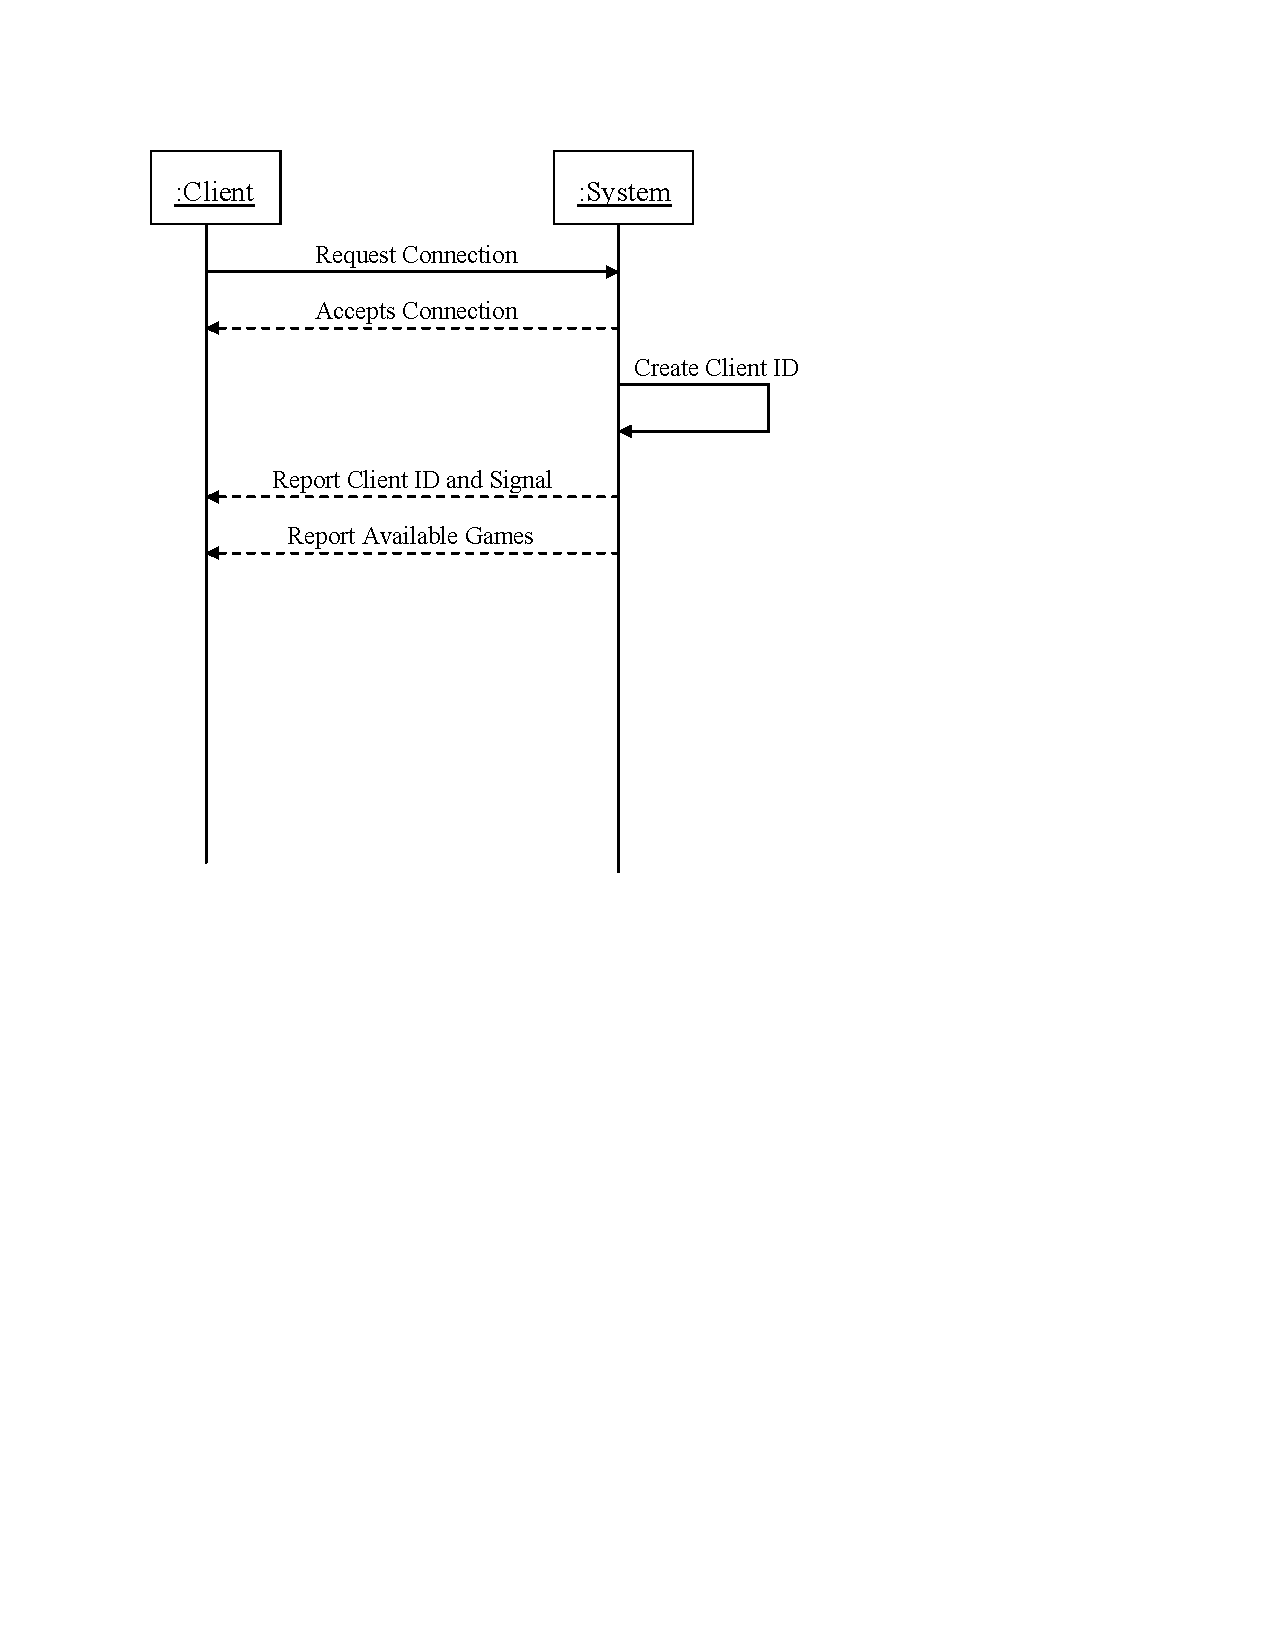
\includegraphics{SSD.pdf} \end{center} 

\section{Nonfunctional Requirements}
\begin{itemize}
\item The desired communication time between a phone and server should be processed and stored with less than a 75 nanosecond lag-time.
\item The server should be able to handle at least 10 simultaneous conversations (games) without failure. 
\item If the server is unable to store game data, we will inform client so that the client may present the user with a message stating that the data will not be stored (high scores, replay information, etc.), but otherwise gameplay will remain unaffected. 
\item We will also plan on having two types of computer-programmed players. One will simply track ball movement, and the other with more randomization. 
\item Ideally we'd have players determine the size of the playing field, and that size would automatically create a ratio that fits to the client interface. 
\end{itemize}
These secondary features will bring out the performance and ability of our server and increase the game options Vir-Pong players are afforded. 

\section{Domain Analysis}
The domain of our problem consists largely of a client, game, and a lobby. We want the lobby, our conceptualization of a server, to connect clients to games.\\
\begin{center}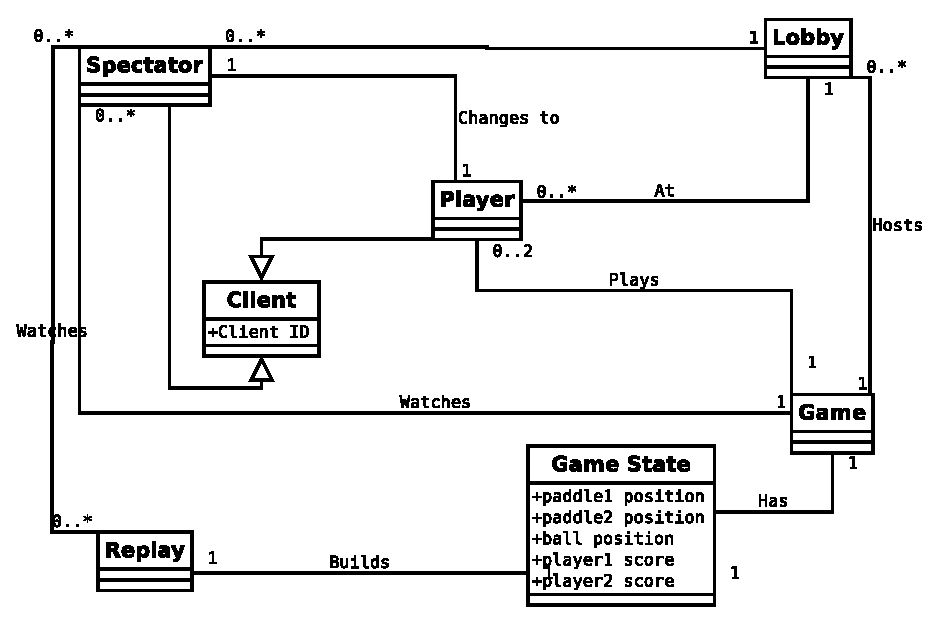
\includegraphics{DomAnaUML.eps} \end{center} 
A client is recognized mainly by the device used in connecting with the lobby. This device is assigned a clientID by the lobby in order to track user interactions with the system. At any one point in time, a client can be either a player or an observer. A client can easily switch between these definitions, but will always retain their clientID while connected. Such is why we have made player and spectators conceptual classes of the generic class client. A theoretically infinite amount of spectators can observe a game, but only two players can play one game. The lobby that connects players and observers to games can host a theoretically infinite amount of games at any one given moment, but all games are tagged back to one lobby. Each game is associated with a single game state. This game state holds the positions of the paddles and the ball. The game state only exists during an instance of the game and, quite essentially, holds the state of a game. Our definition of a game state is the position of paddles and the ball. This game state builds a replay. Any number of spectators can watch any number of these replays. 

\section{Interaction Diagram}

\section{Implementation}
\subsection{Style Guide}
\subsubsection{Whitespace}
The basic indentation is two spaces. Tabs are not to be used at all.
Try to keep lines to 80 characters or less. When wrapping lines, try to indent to line up with a related item on the previous line. Examples: 
\begin{verbatim}
var result = prompt(aMessage,
                    aInitialValue,
                    aCaption);
\end{verbatim}
Lines should not contain trailing spaces, even after binary operators, commas or semicolons.
Separate binary operators with spaces.
Spaces go after commas and semicolons, but not before.
Spaces go after keywords. For example:
\begin{verbatim}
if (x > 0)
\end{verbatim}
One (or two) blank lines between block definitions. Also consider breaking up large code blocks with blank lines.

\subsubsection{Commenting}
Use multi-line comments to explain the purpose behind blocks of code.
Use in-line comments often to clarify actions.

\subsubsection{Symbols}
Function braces can either be on their own line or the open brace on the function declaration, i.e.

\begin{verbatim}
function toOpenWindow(aWindow)
  {
    aWindow.document.commandDispatcher.focusedWindow.focus();  
  }

function toOpenWindow(aWindow) {
    aWindow.document.commandDispatcher.focusedWindow.focus();  
}
\end{verbatim}
Spaces are not necessary inside brackets e.g. parameter lists, array subscripts.
Prefer double quotes, except in in-line event handlers or when quoting with double quotes ie (‘he said, “trouble” ’).
Have braces indented relative to their parent statement.
\subsubsection{Function and Varible Naming}
\begin{itemize}
\item Arguments (parameter names) should be prefixed with the letter a.
\item Event handler functions should be prefixed with the word "on".
\item Function names, local variables and object members have no prefix.
\item Try to declare local variables as near to their use as possible; try to initialize every variable.
\end{itemize}

\subsubsection{JavaScript Features}
Make sure that your code doesn't generate any strict JavaScript warnings, such as:
\begin{itemize}
      	  \item{Duplicate variable declaration}
      	  \item{Mixing return; with return value;}
      	  \item{Trailing comma in JavaScript object declarations}
\end{itemize}    	
If you are unsure if an array value exists, compare the index to the array's length. If you are unsure if an object member exists, use "name" in aObject, or if you are expecting a particular type you may use typeof aObject.name == "function" (or whichever type you are expecting).
Use \{ member: value, ... \} to create a JavaScript object; a useful advantage over new Object() is the ability to create initial properties and use extended JavaScript syntax to define getters and setters.  If having defined a constructor you need to assign default properties it is preferred to assign an object literal to the prototype property. For example,

\begin{verbatim}
function SupportsString(data)
{
  this.data = data;
}
\end{verbatim}
Do not compare booleans to true or false. For example, write if (ioService.offline). Compare objects to null, numbers to 0 or strings to "" if there is chance for confusion.

\subsection{Install Documentation}
\subsubsection{Server}
Requirements:
\begin{itemize}
\item A relatively new machine (read: purchased/built in the last six years or so) running Linux or Mac OS X (These instructions were generated on a machine running Ubuntu 11.10 -- the configuration used for generation of instructions will henceforth be denoted in parentheses).
\item Basic Unix tools will already be installed, but other requirements that may not be present in a standard installation are:
Curl (using 7.21.6)
Git (using 1.7.5.4)
\item Connection to the Internet. 
\end{itemize}
Instructions:
Each line is a unix command, and so each of these commands must be typed into a shell of some sort, such as BASH or ZSH (using BASH). Alternatively, these commands can be easily generated into a BASH shell script quite easily if so desired.

To install node and the node package manager (npm):

\begin{verbatim}
> echo 'export PATH=$HOME/local/bin:$PATH' >> ~/.bashrc
> . ~/.bashrc
> mkdir ~/local
> mkdir ~/node-v0.4.9
> cd ~/node-v0.4.9
> curl http://nodejs.org/dist/node-v0.4.9.tar.gz | tar xz --strip-components=1
> ./configure --prefix=~/local
>make install
>curl http://npmjs.org/install.sh | sh
\end{verbatim}

To install the express web framework and socket.io:

\begin{verbatim}

npm install -g express socket.io #installs express server (expressjs.org) and socket.io
cd <your directory name>
express express-test && cd express-test
npm install -d #resolve dependencies
node app.js #runs test server with node
#point browser to localhost:3000 (default) -- should see welcome message
\end{verbatim}

To run the server:

First, clone the paddle-meister repository using git:

\begin{verbatim}
git clone git://github.com/VirPong/paddle-meister.git
\end{verbatim}

Then, navigate to the socket-test folder and execute:

\begin{verbatim}
node server.js
\end{verbatim}

The server will run at whichever port specified in the PORT variable in server.js. To shutdown the server, press CTRL-C twice.

\subsubsection{MongoDB and Modules}
First we went to mongodb.org and found the path to the most recent 64-bit Linux download. We then put this onto the server using terminal commands: wget [web path]. We then uncompressed the file using the command tar zxvf [file name].tgz.

\begin{verbatim}  
  $wget http://fastdl.mongodb.org/linux/mongodb-linux-x86_64-2.0.1.tgz
  $tar zxvf mongodb-linux-x86_64-2.0.1.tgz
\end{verbatim}

We then installed mongodb using: 

 \begin{verbatim}
  $sudo apt-get install mongodb
\end{verbatim}

After looking over this open-source module, we determined that node-mongodb-native ( https://github.com/christkv/node-mongodb-native )was perfectly suited for our concerns. This module facilitates a connection between mongodb and our server, which uses node. We copied the repository from github using:

\begin {verbatim}
  $git clone git://github.com/christkv/node-mongodb-native.git
\end{verbatim}

However, we ran into a compilation error when attempting to run example code, complaining of the native bson parser not being compiled.
In searching for a solution, we were found another module for mongodb, called mongojs ( https://github.com/gett/mongojs ).Mongojs is actually a wrapper for mongodb-native that allows code to be written in a format almost identical to the mongodb shell API. This allows the code to be condense and clear.
We retrieved node-mongodb-native from github and mongojs was installed via npm with the terminal command:

\begin {verbatim}
  $npm install mongojs
\end{verbatim}

Mongojs allows for very simple, one line connection to the database. Connection in Javascript is as follows: 
\begin {verbatim}
  var db = require('mongojs').connect('database', ['collection']); 
\end{verbatim}
Replace 'database' with the database name you wish to use and 'collection' with the collection name you wish to use. They do not need to exist when you connect. 


\subsection{Algorithms, Data Structures, and Design Patterns}
\subsubsection{Design Pattern}
The node.js server framework is event-driven, so naturally design has been focused around creating and dealing with events.
For example, there are connect, disconnect, updatePaddle, startGame, and other such events that are implemented both server- and client-side.

\subsection{Data Storage}
The data we’re storing is specific to games and the players. We have limited ourselves to usernames, paddle positions, ball positions, scores, and gameIDs. This information will be stored in a noSQL database, mongodb. We have chosen to use a non-relational database because it is not only better for real-time, online, multi-player application, but it has a schema that allows us to directly store and remove Javascript objects without losing any of their structure. 
The main purpose of this data storage is to store information for replays. The replays collection in our database will hold Javascript objects almost identical to those emitted to client during the game. This allows the client a modular way to recreate the game as a replay.
The secondary purpose of this data storage is to cache information that the website will use to interact with their own data. In the gameData collection, we will store usernames, scores, and gameIDs. This information will be transferred to the website’s SQL database.  \\

%The E/R Diagram
\begin{center}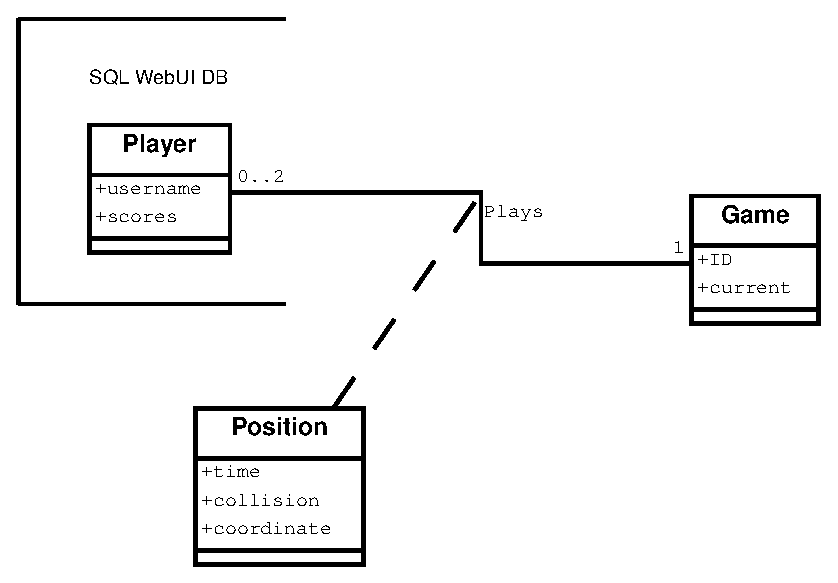
\includegraphics{ERdia.eps} \end{center} 

This diagram is loosely modeled off of an E/R diagram, as a non-relational database typically does not follow relational diagrams. There are two main classes (player and game), and an association complete with a class between them (position). Player is a repository of information that we will communicate with regarding user identity and later update with score information. This information is cached in current game states during a game and will be accessed there. There can be as little as no players a game up to two, with position tracking both the players and the ball. The game section of the document will hold the gameID for tracking and retrieving purposes. The game will also keep track of scores when they are initialized and whenever they are updated. 

BSON documents are the names for the object the database stores. The BSON documents we will be storing are Javascript objects. Initially, we believed that the documents would vary depending on what exactly was occurring during the time of play. However, it soon became apparent that providing the client’s objects almost identical to those the server emits during playtime. We cache these into an array and save this array along with the gameID. A document then looks a bit like this: 
\begin {verbatim}
var replays = { gameID : DATE, replayDocs : [game states] }
\end{verbatim}
The replayDocs is the array of cached game states, and this array looks like this:
\begin{verbatim}
replayDocs = { paddle : paddlePos[player1, player2], ball : ballPos [ballX, ballY],
              scores : score[player1, player2] }
\end{verbatim}

We have set the gameID to Unix time at the start of a game.We initially worried about ensuring uniqueness of gameIDs. We realized it is highly unlikely that there will be duplicates of these IDs.  Player positions, ball positions, and scores are all arrays almost identical to those emitted during gameplay. Player position holds the paddle positions, player one is at zero and player two is at one, the same for scores. Ball have x-coordinates at position zero in the array and y-coordinates at position one. 

It is unnecessary to track collisions as we had first planned. Initially, we were going to simply track paddle positions and run in back through the ball logic and submit it back to the client. However, we have decided it would be best to track the ball position instead of running the paddle position back through the game logic. This way is more efficient and modular.

During gameplay, we cache the desired information into an array, and at the game end we removesave it to the database. When a client requests a game based on its gameID, we retrieve all of the documents with that gameID, sort on the indexes, store it in an array of Javascript objects, and emit the data to the client once.

In this way, we will minimize interaction with the database to the end of a game and client request for replays, allowing us less lag time in our game play and fetching replays.

\subsection{Testing and Verification}

The method used to test our database connection code has primarily consisted of unit testing on the server machine. By using the node-mongodb-native module, any .js files that have calls to the mongodb in them can be run and tested simply by using the ‘node’ command before the file name. Primarily print statements (or, in this case sys.puts(‘ ’); statements) were used to track logical errors. Any compilation on runtime errors were sorted out by referencing the mongodb manuals (as mongojs allows us to write database calls in the mongodb native API) and javascript tutorials. Future integration testing will likely use computer controlled players in games to test data input into the database. After that it will be tested using real player from device inputs.

The method used to test the pong game logic was through the JSBin website. JSBin allows for real time viewing of javascript code and reports errors and warnings in the code as well. From here the server team was able make changes to the code and see how it immediately effected the game logic. JSBin has allowed for learning javascript easier and testing code more efficient.

Server networking was tested primarily with Google Chrome’s JavaScript inspector, as well as the node.js debug mode. There was, of course, plenty of trial-and-error.

\section{Reflections}
\subsection{Technical Challenges}
\begin{itemize}
\item Javascript -- perhaps the most challenging portion of this project was learning and using Javascript. The concepts of Javascript were foriegn to us and we researched tutorials, 
\item Communication -- simple communication between the phones and server was incredibly challenging. Getting the communication to register on both the server and the phone took a great deal of debugging. Extra research yielding progress and allowed communication to flow smoothly. In retrospect, it would have probably been beneficial to just pick the most documented and widely-used communication library and worked through it. That being said, the current communication library has been working well since we broke through the "wall" of problems.
\item Game logic -- the code used as a basis for game logic was not well documented and took a great deal of effort and time to understand the code's implementation, as well as how we could make use of it. It would have probably been better to just write the game logic from scratch, which would not have been too hard since pong was one of the first arcade games ever made.  When the game logic was moved onto the server it could not be easily tested because the server was down after testing and being updated with the code for multiple rooms.  We also relied on the web team in order to view the game and test the logic which forced us to code ot be able to test it in any way for a while after.  The game logic on the server was written using arrays for variables, e.g. paddleSize[x,y] would be the paddle x width and the paddle y height and working with system made it very easy to accidently use y where we wanted x. This lead to several confusing errors in game play that took us a bit of time to correct.
\item Replays -- there were two challenges posed by replays: the repository and communication. After doing research, we determined that we would use a non-relational database; we then choose the most well-documented non-relational database at current: mongodb. Installing and interacting with mongo provided its own challenges: it had its own unique query system and required modules to connect to code. After developing queries and plans, we had to integrate interaction with the database into communication. It was challenging to determine when we would talk to the database. The phones asked us to provide differences in our code. There were also Javascript issues with this. Mongodb automatically stored inputted data as objects, requiring us to cast if we want to interact with this object. 

\end{itemize}

\subsection{Engineering techniques used}
\begin{itemize}
\item Knowing about the software engineering techniques sooner would have been much nicer. We learned about them after we had implimented our code. Without knowing it, we had, with the help of the Andriod mobile development team, created an adaptor to communicate between the server and front-end of the mobil devices.
Moreover, after learning about software engineering techniques, we attempted to impliment our code with high cohesion and low coupling. 
\end{itemize}

\subsection{What we would have done differently}
\begin{itemize}
\item \textbf{Organization and Planning:} If given the opportunity to restart this project, we would start with a great deal more organization and planning. We were all inexperienced in programming a server and we would have benifitted more from clearer initial planning, organization.
\item \textbf{Enthusiasm:} As college students, its hard to devote as much time as necessary to the large-scale products like this, particularly when we don't have eight hours a day to work on coding. However, some of us did not show enough initiative in taking charge of this product and developing it to its fullest.  Most of our ideal features were implimented, but not fully functional. If all the members had put forth their time and energy into the developing and integrating process, our features would likely be fully functional.
\item \textbf{Communication:} All groups have struggled communicating needs and haves accurately, both within and without teams. If we had organized ourselve to talk with each other more often about changes in plans, needs, and new developments the project would have gone more smoothly. Constant communication is essential for a project this size. It was only midway that we actually became organized enough to sit down and communicate across groups.
\end{itemize}

\subsection{Where we would go from here}
\begin{itemize}
\item \textbf {Replays:} If we continued this project, one aspect we would continue building would be replays. At current, our replay functionality is merely a proof of concept. We save game information and can turn around and view game information. However, this is not ideal. We access game information based on the gameIDs, which are long strings of numbers representing Unix Time; but these mean nothing to a user. Ideally we would want them to be able to choose a game based one information a user would likely want to look at - usernames, play time, scores, or date. Moreover, we would like to impliment a bit more features on the replay itself, likely in conjunction with client-side development; these would include setting the replay speed largely consisting of pausing the replay, rewinding the replay, and speeding or slowing down the replaying game. There are also some minor features we would include, such as allowing a player to choose whether or not to save the replay and determining when and what to remove from the repository when memory becomes full. Also, perhaps finding some way to minimize the size of stored replays, at current each game is about 200 MB. 
\end{itemize}


\section{References}
\subsection{Git and Github}
	\begin{itemize}
		\item Git (http://git-scm.com/) is a distributed version control system that is widely-used in the open source community.
		\item Github (http://github.com/) is a web-based hosting service for projects using git. It provides collaboration tools and many other features such as pull requests and commit management that helps small development groups work efficiently.
		\item The current project repository is hosted on github and collaboration will happen through the web-based UI.
	\end{itemize}
\subsection{node.js}
	\begin{itemize}
		\item node.js (http://nodejs.org/) is an easy-to-learn server-side JavaScript server development environment that supports a myriad of different communication protocols such as HTTP, TCP, and WebSockets.
		\item Will be used as the framework for the server.
		\item express (http://expressjs.com/) is a dead-simple web server application written in node.js.
		\item Socket.io (http://socket.io/) is a cross-platform websocket implementation written in JavaScript for server and client that reverts to Flash and AJAX if WebSockets are not enabled on a certain platform.
	\end{itemize}
\subsection{MongoDB}
	\begin{itemize}
		\item MongoDB (http://mongodb.org/) is a scalable open-source non-relational database with strong node.js support.
		\item mongojs (https://github.com/gett/mongojs) is a wrapper for node-mongodb-native that emulates the mongodb shell API
		\item Node-mongodb-native (https://github.com/christkv/node-mongodb-native/) a node module used to facilitate connection between mongodb and node
		\item Will be used as the main database for storing and retrieving game information.
	\end{itemize}

\subsection{Eclipse}
	\begin{itemize}
		\item Eclipse is an Integrated Development Environment written in Java that provides support for many different programming languages and version control systems through plugins -- A git plugin is available, called Egit (http://eclipse.org/egit/).
		\item Most team members will be using Eclipse IDE for development.
	\end{itemize}
\subsection{Google Docs}
	\begin{itemize}
		\item Google Docs (http://docs.google.com/) is an online document processor with tools similar to Microsoft Word, Powerpoint, and others. It allows for collaboration between different users concurrently on the same document.
		\item Will be used for collaboration on internal documents and documentation.
	\end{itemize}
\subsection{Javascript tutorial}
\begin{itemize}
\item An tutorial (http://www.w3schools.com/js/default.asp) used to learn Javascript and compare against compilation errors.
\end{itemize}

\subsection{Reference Code}

\begin{itemize}
\item The pong file that was modified in order to build the game logic of the pong game (https://github.com/garrettdieckmann/human-pong/blob/master/WebUI/site/http/simppong.html)
\item Bits and pieces of Osmus (https://github.com/borismus/osmus) and NodePong (https://github.com/meetar/NodePong) were used in creating a functional networking framework.
\end{itemize}
\subsection{Javascript Style Guide}
\begin{itemize}
\item A Javascript Style Guide created by Neil Rashbrook (http://neil.rashbrook.org/JS.htm ). We referenced and modified it to create a version applicable to our needs.
\end{itemize}
\end{document}
\subsection{JSBin}
\begin{itemize}
\item JS Bin (http://jsbin.com/odiyej/38/edit) allows for editing and testing of JavaScript and HTML, and includes collaborative functionality. 
\end{itemize}
